\documentclass[aspectratio=169,12pt,fleqn]{beamer}
\usetheme{Madrid}
\usecolortheme{dolphin}
\setbeamertemplate{navigation symbols}{}
\usepackage[utf8]{inputenc}
\usepackage[T1]{fontenc}
\usepackage{graphicx}
\usepackage{xcolor}
\usepackage{microtype}
\usepackage{tikz}
\usetikzlibrary{positioning,decorations.pathmorphing}
\usetikzlibrary{calc}
\usepackage{amsmath,amssymb}
\usefonttheme{professionalfonts}


% TikZ "chalk" styles
\tikzset{
  chalk line/.style={
    white, line width=1.1pt,
    decorate, decoration={random steps,segment length=2mm,amplitude=0.5pt}
  },
  chalk box/.style={
    draw=white, rounded corners,
    fill=board!85, % slightly lighter than bg
    inner sep=6pt, text width=4.2cm, align=left,
    chalk line
  },
  chalk arrow/.style={->, chalk line}
}

\usepackage{tikz-cd}

% helper: one proof row that appears starting on overlay #1, #2, ...
\usepackage{array} % in the preamble
% preferred: onscreen-friendly
\newcommand{\prow}[5]{%
  \onslide<#1->{#2} & \onslide<#1->{(#3)} & \onslide<#1->{$#4$} & \onslide<#1->{#5} \\[-0.7ex]
}

\AtBeginSection[]{
  \begin{frame}
    \centering
    \vfill
    \Huge\insertsectionhead
    \vfill
  \end{frame}
}


\title{PHI 201: Week 2}
\subtitle{Supposition \& Hypothetical Reasoning}
\author{Hans Halvorson}
\date{September 15, 2025}


% Define a new column type M{<width>} for math mode
\newcolumntype{M}[1]{>{\(\displaystyle}p{#1}<{\)}}
\begin{document}
\frame{\titlepage}

\renewcommand{\arraystretch}{1.2} % extra row spacing

\begin{frame}[t]{Deducing versus Supposing}
\begin{itemize}
  \item A new kind of rule
  \item A new kind of proof format
\end{itemize}
\end{frame}

\begin{frame}[t]{A simple example}

\begin{block}{Argument}
  \begin{enumerate}
  \item If $P$ then $Q$
  \item If $Q$ then $R$
  \item Therefore, if $P$ then $R$
  \end{enumerate}
\end{block}

\begin{itemize}
\item What licences inferring a \textbf{conditional} statement?
\item Hypothetical thinking: Supposing
\end{itemize}
\end{frame}

\begin{frame}[t]{How to prevent mistakes when supposing}
\begin{itemize}
  \item Repaying your debts
  \item If $P$ then $Q$
  \item If $Q$ then $R$
\end{itemize}
\end{frame}

\section{Keeping track of assumptions}


\begin{frame}[t]{Rule of Assumptions (\textsc{A})}
\begin{block}{Form of the rule}
\[
\begin{array}{llll}
n & (n)\;\varphi & &  \text{A}
\end{array}
\]
\end{block}

\begin{block}{Explanation}
\begin{itemize}
\item On line $(n)$, you may write any formula $\varphi$.
\item The dependency of line $(n)$ is its own line number $n$.
\item The justification is marked \textsc{A} (Assumption).
\end{itemize}
\end{block}
\end{frame}

\begin{frame}[t]{$\wedge$-Introduction ($\wedge$\textsc{I})}
  \begin{block}{Form of the rule}
  \[
\begin{array}{c c M{6cm} l l}
  \Delta & (m) & P &     & \\
  \Gamma & (n) & Q &     & \\[6pt]
  \Delta,\Gamma & (k) & P \wedge Q & & m,n \ \wedge\mathrm{I}
\end{array}
\]  

\end{block}

\begin{block}{Explanation}
\begin{itemize}
\item If you have $P$ on line $m$ (with dependencies $\Delta$), and
  $Q$ on line $n$ (with dependencies $\Gamma$), then you may infer
  $P\wedge Q$.
\item The new line $k$ depends on all assumptions of both lines, i.e.\
  the union of $\Delta$ and $\Gamma$.
\item The justification cites both lines: $m,n$ $\wedge$I
\end{itemize}
\end{block}
\end{frame}

\begin{frame}[t]{$\wedge$-Elimination ($\wedge$\textsc{E})}
  \begin{block}{Form of the rule}
  \[
\begin{array}{c c M{6cm} l l}
  \Delta & (m) & P \wedge Q & & \\[6pt]
  \Delta & (k) & P  & & m \ \wedge\mathrm{E}
\end{array}
\]
  \end{block}

  \begin{block}{Explanation}
  \begin{itemize}
  \item If you have $P \wedge Q$ on line $m$ (with dependencies $\Delta$), you may infer either conjunct.  
  \item The new line $k$ carries exactly the same dependency set $\Delta$.  
  \item The justification cites line $m$: $m$ $\wedge$E.
  \end{itemize}
  \end{block}
\end{frame}

\begin{frame}{Keeping track of dependencies}

  \centering\bigskip
  \begin{tabular}{>{\raggedleft\arraybackslash}p{1.5cm} >{\centering\arraybackslash}p{1.0cm} p{5cm} >{\raggedright\arraybackslash}p{3.5cm}}
\textbf{Deps} & \textbf{Line} & \textbf{Formula} & \textbf{Justification} \\ \hline 
1 & (1) & $\mathit{P} \land \mathit{Q}$ & A \\
1 & (2) & $\mathit{P}$ & 1 $\wedge$E \\
1 & (3) & $\mathit{Q}$ & 1 $\wedge$E \\
1 & (4) & $\mathit{Q} \land \mathit{P}$ & 3,2 $\wedge$I \\
\end{tabular}

\end{frame}

\begin{frame}[t]{$\vee$-Introduction ($\vee$\textsc{I})}
  \begin{block}{Form of the rule}
  \[
\begin{array}{c c M{6cm} l l}
  \Delta & (m) & P & & \\[6pt]
  \Delta & (k) & P \vee Q & & m \ \vee\mathrm{I}
\end{array}
\]
  \end{block}

  \begin{block}{Explanation}
  \begin{itemize}
  \item If you have $P$ on line $m$ (with dependencies $\Delta$), you may infer a disjunction $P \vee Q$ on a new line.  
  \item You are free to introduce any formula $Q$ as the other disjunct.  
  \item The new line $k$ carries the same dependencies $\Delta$.  
  \item The justification cites the original line: $m$ $\vee$E.
  \end{itemize}
  \end{block}
\end{frame}

\begin{frame}[t]{Modus Ponens (MP)}
  \begin{block}{Form of the rule}
  \[
\begin{array}{c c M{6cm} l l}
  \Delta & (m) & P\to Q & & \\
  \Gamma & (n) & P  & & \\[6pt]
  \Delta,\Gamma & (k) & Q & & m,n \ \mathrm{MP}
\end{array}
\]
  \end{block}

  \begin{block}{Explanation}
  \begin{itemize}
  \item If you have $P\to Q$ on line $m$ (with dependencies $\Delta$)
    and $P$ on line $n$ (with dependencies $\Gamma$), then you may
    infer $Q$.
  \item The new line $k$ carries the union of dependencies: $\Delta \cup \Gamma$.  
  \item The justification cites both lines: $m,n$ MP.
  \end{itemize}
  \end{block}
\end{frame}

\begin{frame}[t]{Modus Tollens (MT)}
  \begin{block}{Form of the rule}
  \[
\begin{array}{c c M{6cm} l l}
  \Delta & (m) & P\to Q & & \\
  \Gamma & (n) & \neg Q & & \\[6pt]
  \Delta,\Gamma & (k) & \lnot P & & m,n \ \mathrm{MT}
\end{array}
\]
  \end{block}

  \begin{block}{Explanation}
  \begin{itemize}
  \item If you have $P\to Q$ on line $m$ (with dependencies $\Delta$),
    and $\neg Q$ on line $n$ (with dependencies $\Gamma$), then you
    may infer $\neg P$.
  \item The new line $k$ depends on all assumptions of both lines,
    i.e.\ $\Delta \cup \Gamma$.
  \item The justification cites both lines: $m,n$ MT.
  \end{itemize}
  \end{block}
\end{frame}

\begin{frame}{Keeping track of dependencies}

  \begin{tabular}{>{\raggedleft\arraybackslash}p{1.5cm} >{\centering\arraybackslash}p{1.0cm} p{5cm} >{\raggedright\arraybackslash}p{3.5cm}}
\textbf{Deps} & \textbf{Line} & \textbf{Formula} & \textbf{Justification} \\ \hline
1 & (1) & $\mathit{P} \to (\mathit{Q} \to \mathit{R}$) & A \\
2 & (2) & $\lnot \mathit{R} \land \mathit{P}$ & A \\
2 & (3) & $\mathit{P}$ & 2 $\wedge$E \\
1,2 & (4) & $\mathit{Q} \to \mathit{R}$ & 1,3 MP \\
2 & (5) & $\lnot \mathit{R}$ & 2 $\wedge$E \\
1,2 & (6) & $\lnot \mathit{Q}$ & 4,5 MT \\
\end{tabular}



\end{frame}

\begin{frame}[t]{Double Negation (DN)}
  \begin{block}{Form of the rule}
  \[
\begin{array}{c c M{2.5cm} l l}
  \Delta & (m) & P & & \\[6pt]
  \Delta & (k) & \lnot\lnot P & & m \ \mathrm{DN}
\end{array}
\qquad\qquad
\begin{array}{c c M{2.5cm} l l}
  \Delta & (m) & \lnot\lnot P & & \\[6pt]
  \Delta & (k) & P & & m \ \mathrm{DN}
\end{array}
\]
  \end{block}

  \begin{block}{Explanation}
  \begin{itemize}
  \item From $P$ you may infer $\lnot\lnot P$, or from $\lnot\lnot P$ you may infer $P$.  
  \item In either case, the dependency set $\Delta$ is preserved.  
  \item The justification cites the relevant line: $m$ DN.
  \end{itemize}
  \end{block}
\end{frame}

%% now give an example of a proof from last week 

\begin{frame}[t]{Summary}

  \begin{itemize}
  \item For all of the deducing rules (Chapter 2), the dependencies on
    the new line are the aggregate of the dependencies of the cited
    lines.
  \item Dependency order does not matter \newline 
    $1,2$ is the same as $2,1$
  \item Dependency duplication does not matter \newline
    No difference between $1,1$ and $1$
  \end{itemize}



\end{frame}

\begin{frame}[t]{Summary}

  \begin{block}{Key Idea}
  Each proof line makes a statement:
  \[
    \begin{array}{c c M{2.5cm} l l} 
      \Delta & (n) & P & \ast 
    \end{array}
  \]
  \emph{The sentences on lines $\Delta$ logically imply $P$.}
  \end{block}

  \begin{alertblock}{Watch Out!}
  Hint: keep an eye out for suspicious lines, for example:
  \[
    \begin{array}{c c M{2.5cm} l l}
      1 & (1) & P & \mathrm{A} \\
        & \vdots & & \\ 
      1 & (n) & P \wedge Q &
    \end{array}
  \]
  \end{alertblock}

\end{frame}


\section{Conditional proof}


\begin{frame}[t]{Conditional Proof (CP)}
  \begin{block}{Form of the rule}
  \[
\begin{array}{c c M{6cm} l l}
  n           & (n) & P               & & A \\[6pt]
  \Delta      & (m) & Q               & &   \\[6pt]
  \Delta \setminus \{n\} & (k) & P \to Q & & n,m\ \mathrm{CP}
\end{array}
  \]
  \end{block}

  \begin{block}{Explanation}
  \begin{itemize}
    \item Start a subproof at line $n$ by assuming $P$ (\textsc{A}).
    \item Derive $Q$ on line $m$ with dependencies $\Delta$.
    \item By \textsc{CP}, infer $P\to Q$ on line $k$; its dependencies
      are $\Delta\setminus\{n\}$ (discharge $n$).
  \end{itemize}
  \end{block}
\end{frame}



\begin{frame}{Conditional proof}

  \centering
  \bigskip 

\begin{tabular}{>{\raggedleft\arraybackslash}p{1.6cm} >{\centering\arraybackslash}p{1cm} p{5cm} >{\raggedright\arraybackslash}p{3.5cm}}
\textbf{Deps} & \textbf{Line} & \textbf{Formula} & \textbf{Justification} \\ \hline
1 & (1) & $\mathit{P} \to \mathit{Q}$ & A
\\ 
2 & (2) & $\mathit{Q} \to \mathit{R}$ & A
\\ 
3 & (3) & $\mathit{P}$ & A
\\ 
1,3 & (4) & $\mathit{Q}$ & 1,3 MP
\\ 
1,2,3 & (5) & $\mathit{R}$ & 2,4 MP 
\\ 
1,2 & (6) & $\mathit{P} \to \mathit{R}$ & 3,5 CP
\end{tabular}

\end{frame}

\begin{frame}{Conditional proof}

  \centering
  \bigskip

\begin{tabular}{>{\raggedleft\arraybackslash}p{1.5cm} >{\centering\arraybackslash}p{1cm} p{6cm} >{\raggedright\arraybackslash}p{3.5cm}}
\textbf{Deps} & \textbf{Line} & \textbf{Formula} & \textbf{Justification} \\ \hline
1 & (1) & $(\mathit{P} \land \mathit{Q})\to \mathit{R}$ & A 
\\ 
2 & (2) & $\mathit{P}$ & A
\\ 
3 & (3) & $\mathit{Q}$ & A
\\ 
2,3 & (4) & $\mathit{P} \land \mathit{Q}$ & 2,3 $\wedge$I 
\\ 
1,2,3 & (5) & $\mathit{R}$ & 1,4 MP 
\\ 
1,2 & (6) & $\mathit{Q} \to \mathit{R}$ & 3,5 CP
\\ 
1 & (7) & $\mathit{P} \to (\mathit{Q} \to \mathit{R})$ & 2,6 CP 
\\ 
\end{tabular}
  


\end{frame}

\begin{frame}{Contrapositive}

  \centering
  \bigskip 
\begin{tabular}{>{\raggedleft\arraybackslash}p{1.5cm} >{\centering\arraybackslash}p{1cm} p{4cm} >{\raggedright\arraybackslash}p{3.5cm}}
\textbf{Deps} & \textbf{Line} & \textbf{Formula} & \textbf{Justification} \\ \hline
1 & (1) & $\mathit{P} \to \mathit{Q}$ & Assumption
\\ 
2 & (2) & $\lnot \mathit{Q}$ & A
\\ 
1,2 & (3) & $\lnot \mathit{P}$ & 1,2 MT 
\\ 
1 & (4) & $\lnot \mathit{Q} \to \lnot \mathit{P}$ & 2,3 CP 
\end{tabular}



\end{frame}


% example of P\wedge Q\to R \vdash P\to (Q\to R)

% example of P\wedge Q\to P


% example of P \to P

\begin{frame}[t]{Proofs without premises}

  \centering\bigskip

  \begin{tabular}{>{\raggedleft\arraybackslash}p{1.5cm} >{\centering\arraybackslash}p{1cm} p{4cm} >{\raggedright\arraybackslash}p{3.5cm}}
\textbf{Deps} & \textbf{Line} & \textbf{Formula} & \textbf{Justification} \\ \hline
    1 & (1) & $P\wedge Q$ & A  \\
    1 & (2) & $P$ & 1 $\wedge$E \\  
      & (3) & $(P\wedge Q)\to P$ & 1,2 CP \end{tabular}

  \end{frame}

  \begin{frame}{DeMorgan's rule}

    \centering\bigskip

\begin{tabular}{>{\raggedleft\arraybackslash}p{1.5cm} >{\centering\arraybackslash}p{1cm} p{4cm} >{\raggedright\arraybackslash}p{3.5cm}}
\textbf{Deps} & \textbf{Line} & \textbf{Formula} & \textbf{Justification} \\ \hline
1 & (1) & $\lnot (\mathit{P} \lor \mathit{Q})$ & Assumption
\\ 
2 & (2) & $\mathit{P}$ & A
\\ 
2 & (3) & $\mathit{P} \lor \mathit{Q}$ & 2 $\vee$I 
\\ 
$\varnothing$ & (4) & $\mathit{P} \to (\mathit{P} \lor \mathit{Q}$) &
                                                                      2,3
                                                                      CP
                                                                      
\\ 
1 & (5) & $\lnot \mathit{P}$ & 4,1 MT 
\end{tabular}
  
\end{frame}

\begin{frame}[t]{Proofs without premises}

  \centering\bigskip

  \begin{tabular}{>{\raggedleft\arraybackslash}p{1.6cm} >{\centering\arraybackslash}p{1cm} p{4cm} >{\raggedright\arraybackslash}p{3.5cm}}
\textbf{Deps} & \textbf{Line} & \textbf{Formula} & \textbf{Justification} \\ \hline
  1 & (1) & $P$ & A  \\
     & (2) & $P\to P$           & 1,1 CP \end{tabular}

\end{frame}

  

\begin{frame}[t]{Conditional proof}

  \centering\bigskip 

  \begin{tabular}{>{\raggedleft\arraybackslash}p{1.5cm} >{\centering\arraybackslash}p{1cm} p{6cm} >{\raggedright\arraybackslash}p{3.5cm}}
\textbf{Deps} & \textbf{Line} & \textbf{Formula} & \textbf{Justification} \\ \hline
  1 & (1) & $P \wedge Q$ & A  \\
  1 & (2) & $P$           & 1 $\wedge$E  \\
    1 & (3) & $Q$           & 1 $\wedge$E  \\
    & (4) & $P\to Q$     & 2,3 CP \end{tabular}

\end{frame}

%% later

\section{Disjunction elimination}

\begin{frame}{Disjunction Elimination ($\lor$E)}
\centering
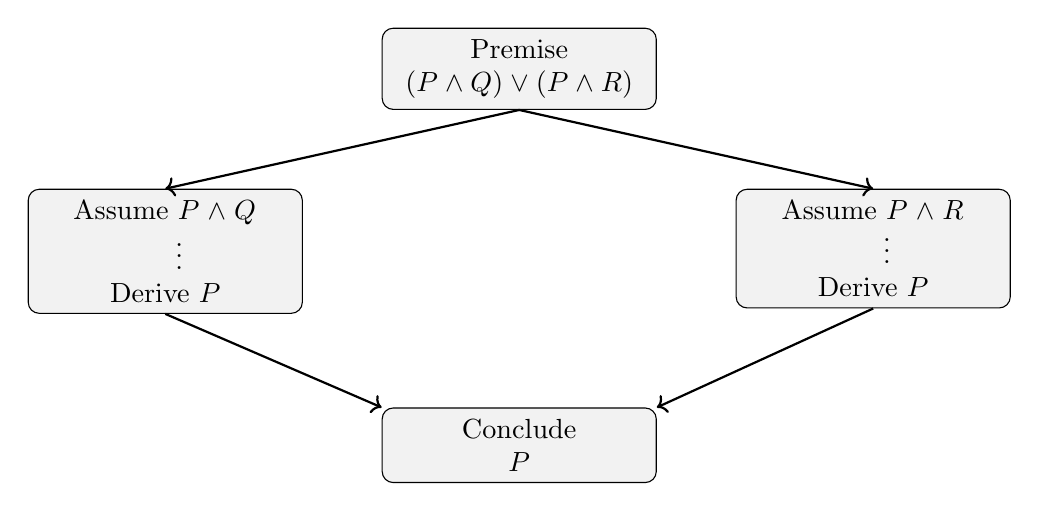
\begin{tikzpicture}[
  node distance=1.0cm and 1.0cm,
  box/.style={draw, rounded corners, fill=gray!10, inner sep=4pt, text width=3.2cm, align=center},
  arrow/.style={->, thick}
]

% Premise
\node[box] (prem) {Premise \\ $(P\wedge Q)\vee (P\wedge R)$};

% Subproofs side by side
\node[box, below left=of prem] (left) {
  Assume $P\wedge Q$ \\
  \quad $\vdots$ \\
  Derive $P$
};
\node[box, below right=of prem] (right) {
  Assume $P\wedge R$ \\
  \quad $\vdots$ \\
  Derive $P$
};

% Conclusion directly beneath both
% \node[box, below=of $(left)!0.5!(right)$] (concl) {$R$};
\node[box, below=2cm of $(left)!0.5!(right)$] (concl) {Conclude \\ $P$};

% Arrows
\draw[arrow] (prem.south) -- (left.north);
\draw[arrow] (prem.south) -- (right.north);
\draw[arrow] (left.south) -- (concl.north west);
\draw[arrow] (right.south) -- (concl.north east);

\end{tikzpicture}
\end{frame}

\begin{frame}{Disjunction elimination}

  \centering\bigskip

  \begin{tabular}{>{\raggedleft\arraybackslash}p{1.5cm} >{\centering\arraybackslash}p{1cm} p{6cm} >{\raggedright\arraybackslash}p{3.5cm}}
\textbf{Deps} & \textbf{Line} & \textbf{Formula} & \textbf{Justification} \\ \hline
1 & (1) & $(\mathit{P} \land \mathit{Q})\lor (\mathit{P} \land \mathit{R})$ & A
\\ 
2 & (2) & $\mathit{P} \land \mathit{Q}$ & A
\\ 
    2 & (3) & $\mathit{P}$ & 2 $\wedge$E 
\\ 
4 & (4) & $\mathit{P} \land \mathit{R}$ & A
\\ 
4 & (5) & $\mathit{P}$ & 4 $\wedge$E 
\\ 
1 & (6) & $\mathit{P}$ & 1,2,3,4,5 $\vee$E 
\end{tabular}

\end{frame}

\begin{frame}{Disjunction Elimination ($\lor$E)}
\centering
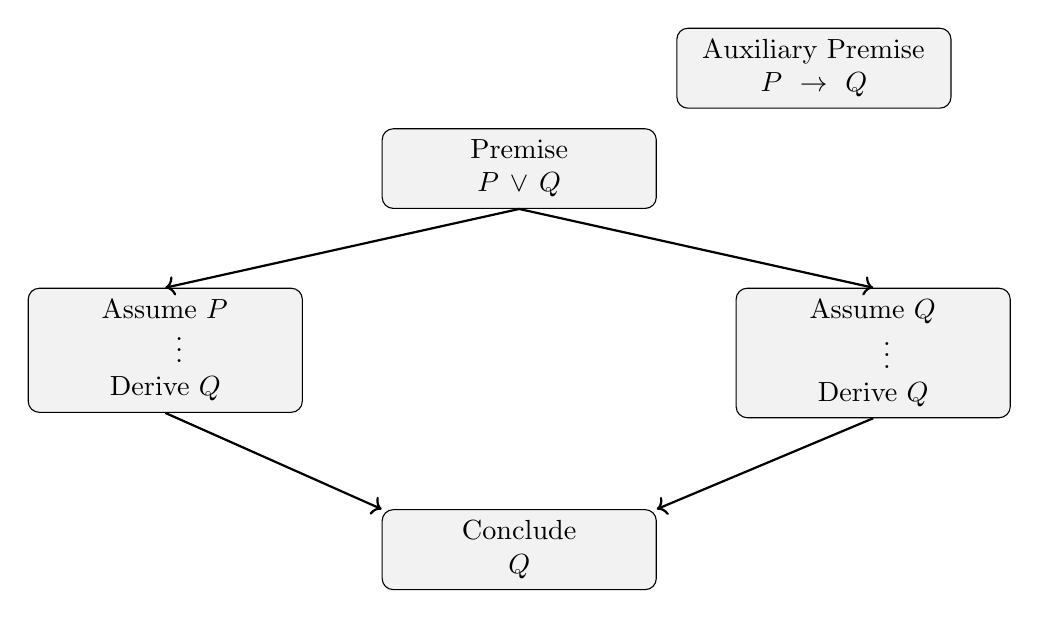
\begin{tikzpicture}[
  node distance=1.0cm and 1.0cm,
  box/.style={draw, rounded corners, fill=gray!10, inner sep=4pt, text width=3.2cm, align=center},
  arrow/.style={->, thick}
]

% Premise
\node[box] (prem) {Premise \\ $P\vee Q$};

\node[box, above right=0.35cm of prem] {Auxiliary Premise \\ $P\to Q$};

% Subproofs side by side
\node[box, below left=of prem] (left) {
  Assume $P$ \\
  \quad $\vdots$ \\
  Derive $Q$
};
\node[box, below right=of prem] (right) {
  Assume $Q$ \\
  \quad $\vdots$ \\
  Derive $Q$
};

% Conclusion directly beneath both
% \node[box, below=of $(left)!0.5!(right)$] (concl) {$R$};
\node[box, below=2cm of $(left)!0.5!(right)$] (concl) {Conclude \\ $Q$};

% Arrows
\draw[arrow] (prem.south) -- (left.north);
\draw[arrow] (prem.south) -- (right.north);
\draw[arrow] (left.south) -- (concl.north west);
\draw[arrow] (right.south) -- (concl.north east);

\end{tikzpicture}


\end{frame}





\begin{frame}{Disjunction elimination}

\centering\bigskip   
  \begin{tabular}{>{\raggedleft\arraybackslash}p{1.5cm} >{\centering\arraybackslash}p{1cm} p{6cm} >{\raggedright\arraybackslash}p{3.5cm}}
\textbf{Deps} & \textbf{Line} & \textbf{Formula} &
                                                   \textbf{Justification} \\ \hline
1 & (1) & $\mathit{P} \to \mathit{Q}$ & A
\\ 
2 & (2) & $\mathit{P} \lor \mathit{Q}$ & A
\\ 
3 & (3) & $\mathit{P}$ & A
\\ 
1,3 & (4) & $\mathit{Q}$ & 1,3 MP
\\ 
5 & (5) & $\mathit{Q}$ & A
\\ 
1,2 & (6) & $\mathit{Q}$ & 2,3,4,5,5 $\vee$E
\\ 
\end{tabular}



\end{frame}

\begin{frame}{Disjunction elimination}

\centering\bigskip 
\begin{tabular}{>{\raggedleft\arraybackslash}p{1.5cm} >{\centering\arraybackslash}p{1cm} p{4cm} >{\raggedright\arraybackslash}p{3.5cm}}
\textbf{Deps} & \textbf{Line} & \textbf{Formula} & \textbf{Justification} \\ \hline
1 & (1) & $\mathit{P} \lor \mathit{P}$ & A
\\ 
2 & (2) & $\mathit{P}$ & A
\\ 
1 & (3) & $\mathit{P}$ & 1,2,2,2,2 $\vee$E
\end{tabular}

\end{frame}

  




\section{Subtleties of conditional proof}

\begin{frame}[t]{Positive paradox}

  \centering  
  \bigskip
  \begin{tabular}{>{\raggedleft\arraybackslash}p{1.5cm}
    >{\centering\arraybackslash}p{1cm} p{4cm} >{\raggedright\arraybackslash}p{3.5cm}}
\textbf{Deps} & \textbf{Line} & \textbf{Formula} & \textbf{Justification} \\ \hline
1 & (1) & $\mathit{Q}$ & A
\\ 
2 & (2) & $\mathit{P}$ & A
\\ 
1 & (3) & $\mathit{P} \to \mathit{Q}$ & 2,1 CP
\end{tabular}



\end{frame}

\begin{frame}[t]{Negative paradox}

  \centering
  \renewcommand{\arraystretch}{1.2} % extra row spacing
  \bigskip

  \begin{tabular}{>{\raggedleft\arraybackslash}p{1.5cm}
    >{\centering\arraybackslash}p{1cm}
                p{4cm}
                >{\raggedright\arraybackslash}p{3cm}}
\textbf{Deps} & \textbf{Line} & \textbf{Formula} & \textbf{Justification} \\
\hline
1   & (1) & $\lnot P$         & A \\
2   & (2) & $P$               & A \\
3   & (3) & $\lnot Q$         & A \\
2   & (4) & $\lnot Q \to P$   & 3,2 CP \\
1,2 & (5) & $\lnot\lnot Q$    & 4,1 MT \\
1,2 & (6) & $Q$               & 5 DN \\
1   & (7) & $P \to Q$         & 2,6 CP 
\end{tabular}
\end{frame}

\begin{frame}{Ex Falso Quodlibet}

  \centering\bigskip

  \begin{tabular}{>{\raggedleft\arraybackslash}p{1.0cm} >{\centering\arraybackslash}p{1cm} p{4cm} >{\raggedright\arraybackslash}p{3.5cm}}
\textbf{Deps} & \textbf{Line} & \textbf{Formula} & \textbf{Justification} \\ \hline
1 & (1) & $\mathit{P}$ & A
\\ 
2 &  (2) & $\lnot \mathit{P}$ & A
\\ 
3 & (3) & $\lnot \mathit{Q}$ & Assumption
\\ 
2 & (4) & $\lnot \mathit{Q} \to \lnot \mathit{P}$ & 3,2 CP 
\\ 
1 & (5) & $\lnot \lnot \mathit{P}$ & 1 DN
\\ 
1,2 & (6) & $\lnot \lnot \mathit{Q}$ & 4,5 MT
\\ 
1,2 & (7) & $\mathit{Q}$ & 6 DN
\end{tabular}



\end{frame}

\begin{frame}{Material conditional}
\centering
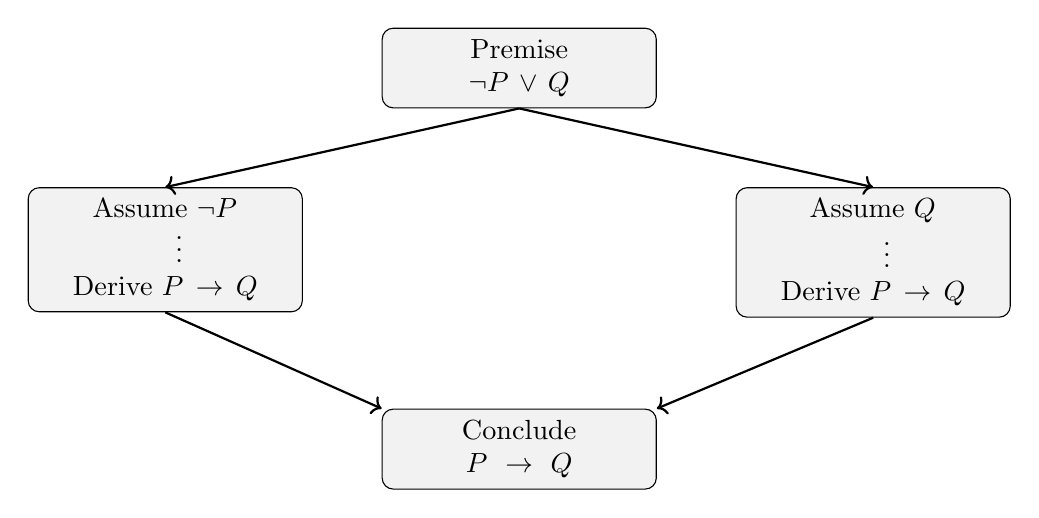
\begin{tikzpicture}[
  node distance=1.0cm and 1.0cm,
  box/.style={draw, rounded corners, fill=gray!10, inner sep=4pt, text width=3.2cm, align=center},
  arrow/.style={->, thick}
]

% Premise
\node[box] (prem) {Premise \\ $\neg P\vee Q$};

% Subproofs side by side
\node[box, below left=of prem] (left) {
  Assume $\neg P$ \\
  \quad $\vdots$ \\
  Derive $P\to Q$
};
\node[box, below right=of prem] (right) {
  Assume $Q$ \\
  \quad $\vdots$ \\
  Derive $P\to Q$
};

% Conclusion directly beneath both
% \node[box, below=of $(left)!0.5!(right)$] (concl) {$R$};
\node[box, below=2cm of $(left)!0.5!(right)$] (concl) {Conclude \\
  $P\to Q$};

% Arrows
\draw[arrow] (prem.south) -- (left.north);
\draw[arrow] (prem.south) -- (right.north);
\draw[arrow] (left.south) -- (concl.north west);
\draw[arrow] (right.south) -- (concl.north east);

\end{tikzpicture}


\end{frame}


%% To Do: It doesn't help to require that the assumption/antecedent
%% dependency occurs among the dependencies of the consequent

\begin{frame}{Summary}

  \begin{itemize}
  \item From now on, proofs consist of \textbf{four} columns.
  \item For the deducing rules, we collect dependency numbers from the
    cited lines.
  \item \textbf{Conditional proof} allows us to derive a conditional
    statement from a ``subproof'' in which we make a new assumption.
  \item \textbf{Disjunction elimination} allows us to draw a
    conclusion from a disjunction if we can draw it from each disjunct
    separately. \end{itemize}

\end{frame}




\end{document}
%%% Local Variables:
%%% mode: latex
%%% TeX-master: t
%%% End:
